\section{Software}
Im Folgenden soll ein grober Überblick über die Software gegeben werden die Im Zuge des Proseminars entwickelt wurde. Dieses Kapitel soll als Einarbeitungs- und eventuelle Weiterentwicklungshilfe dienen. Allerdings wird hier die Software nicht in jedem Detail beschrieben, Zu tieferen Einsichtgen in die Software empfehlen wir entsprechend den Code und die enthaltenen Kommentare zu studieren.
\\
\\
Zuerst kam die Frage auf, wie die Daten vom Sensor möglichst einfach an das Handy gelangen können. Da wir durch den Sensor auf die Verwendung der Bluetooth-Schnittstelle festgelegt waren, welche gerade in Gebäuden keine allzu große Reichweite hat, haben wir uns entschieden eine Zwischenstation einzubauen. Diese soll sich auf das lokale WLan verbinden können, welches in diesem Entwicklungsschritt noch die gesamte Einsatzfläche des Systems abdecken muss. \\
Darüber hinaus dient diese Zwischenstation als Server zum Speichern und Verarbeiten der vom Sensor erhaltenen Daten und bietet eine allgemeine Schnittstelle zur Verfügung, welche von beliebigen Anwendungen verwendet werden kann.
\subsection{Gesamtarchitektur}
\begin{figure}[htb] 
	\centerline{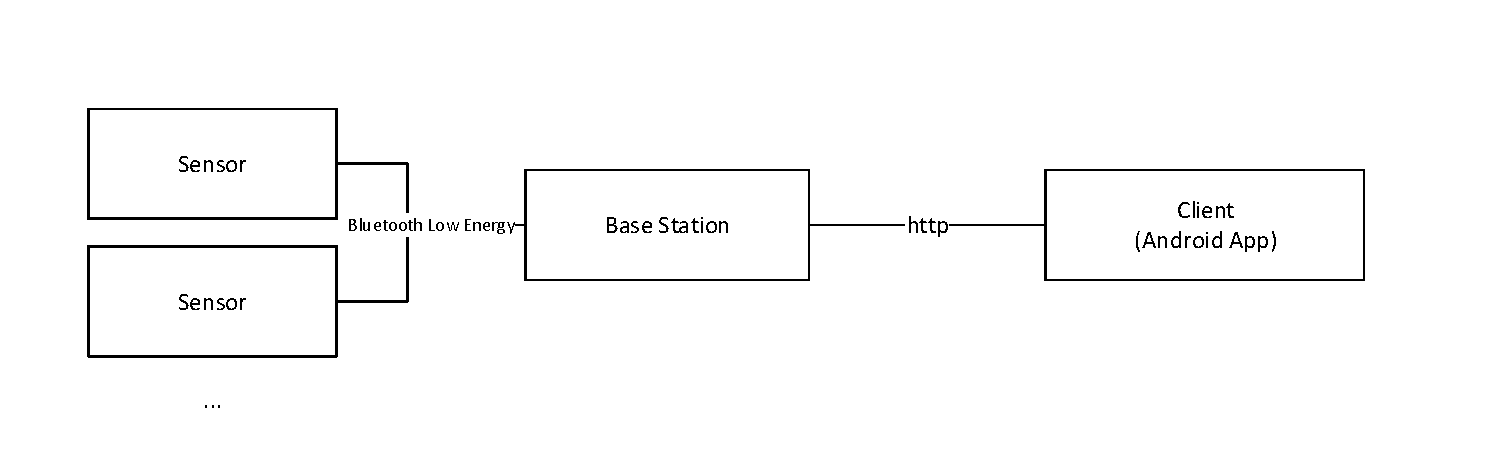
\includegraphics[scale=.5]{Architektur/dryR_complete.pdf}}
	\caption{Das Gesamtschema des Systems.}
\end{figure}

Das Gesamtsystem ist recht einfach gehalten, kann aber durch den modularen Aufbau einfach erweitert werden. Als zentrale Stelle ist die Basisstation vorgesehen, welche über BLE mit den Sensoren kommuniziert. Die Ergebnisse können von einem Client (der Android-Applikation) über eine html-Schnittstelle abgefragt werden.
\subsection{Basisstation}
\begin{figure}[htb] 
	\centerline{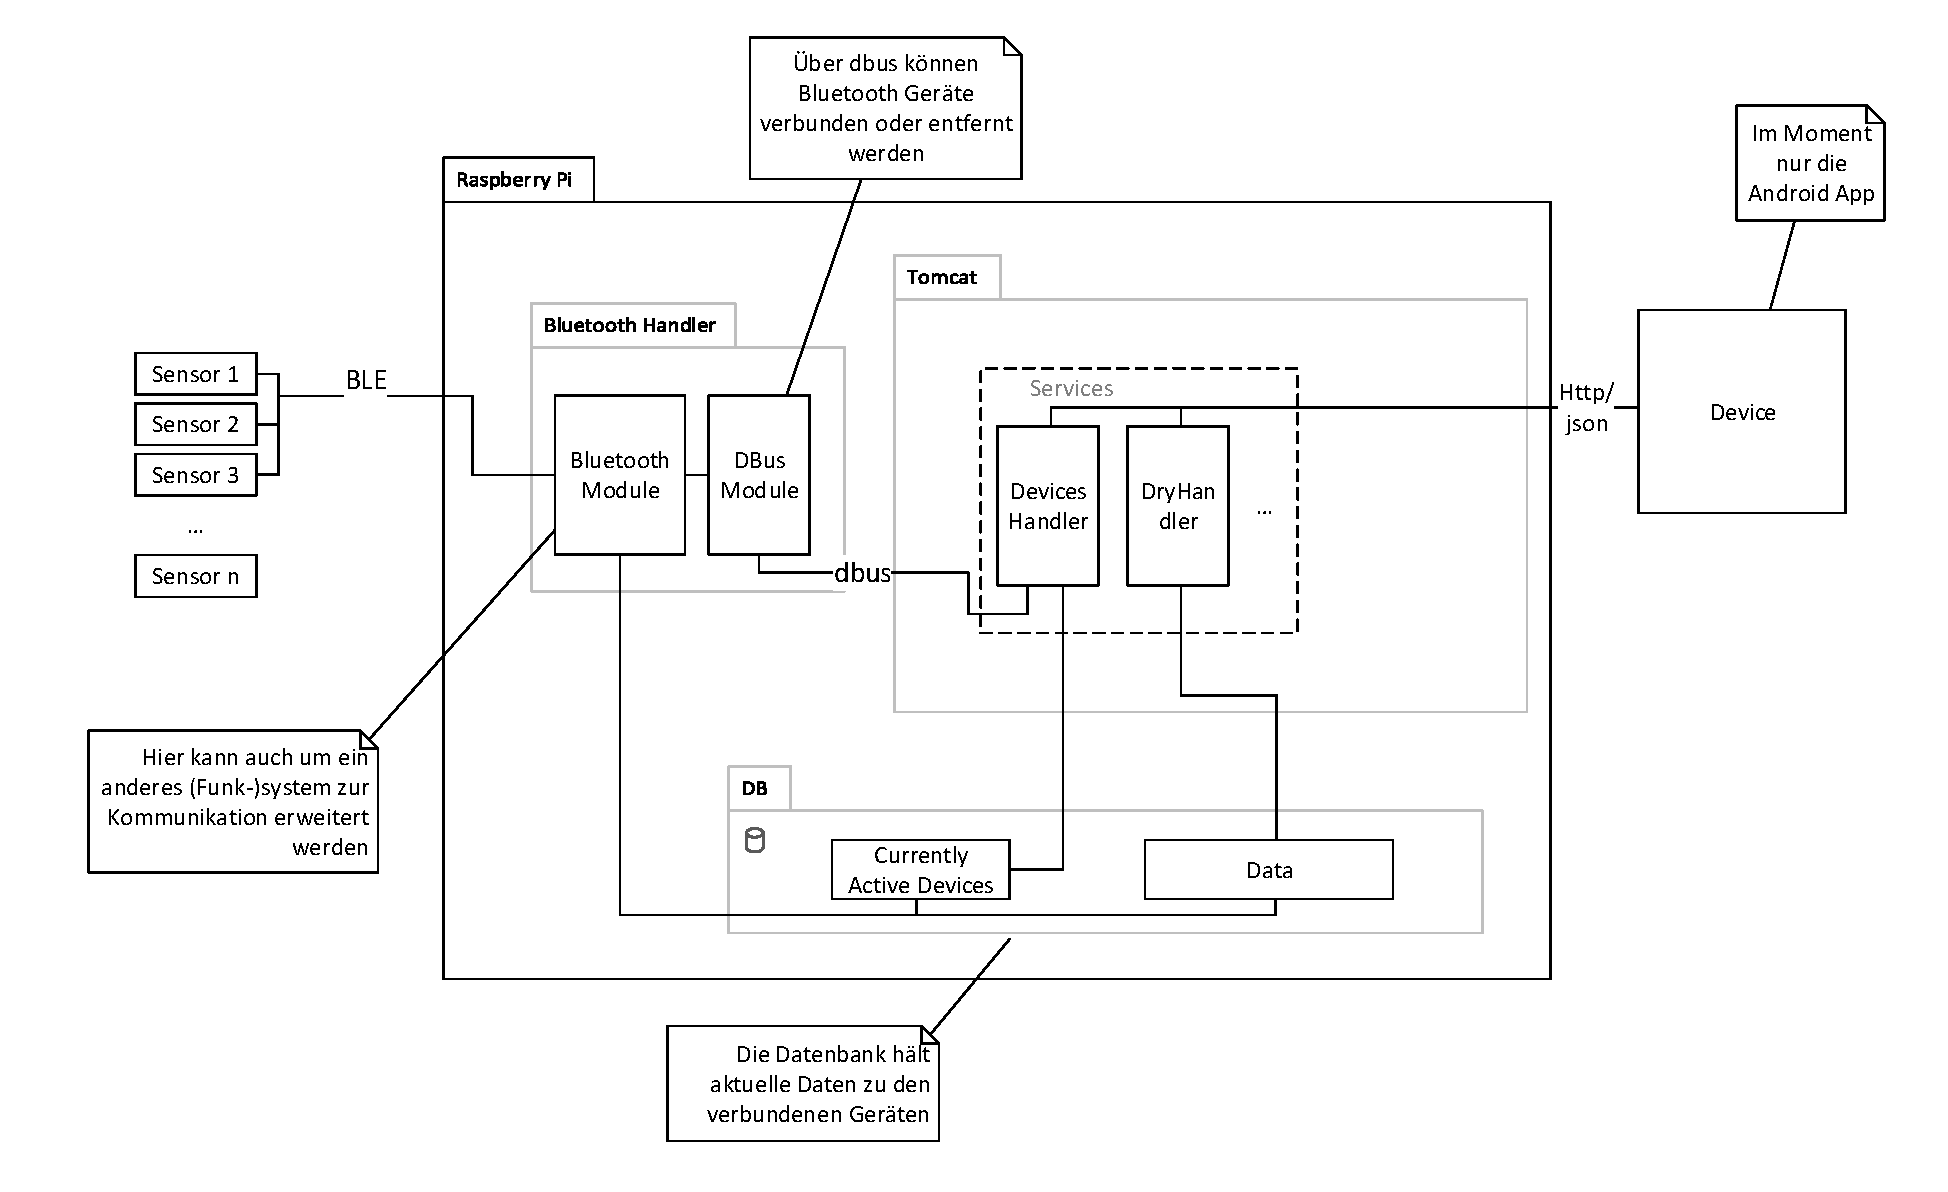
\includegraphics[scale=.4]{Architektur/BaseStation_v2.pdf} }
	\caption{Der Aufbau der Basisstation.}
\end{figure}

Die Basisstation verbindet Datenaggregation, -haltung und -verarbeitung. Dazu verwendet sie eine Oracle MySQL\footnote{http://www.oracle.com/de/products/mysql/overview/index.html} Datenbank, in welche die Sensordaten direkt geschrieben werden und später von den von einem Apache Tomcat\footnote{http://tomcat.apache.org/} Server bereit gestellten Servlets gelesen werden. Dadurch ist es einfach möglich, auch andere Technologien und Sensoren einzubinden, da die entsprechenden Ergebnisse einfach in die Datenbank geschrieben werden und von dort aus weiterverarbeitet werden können.\\
Die Kommunikation zwischen Tomcat-Server und dem Haskell Bluetooth Handler erfolgt dabei über die D-Bus Schnittstelle. So können etwa Geräte auf Anfrage gepairt werden.
\subsubsection{Haskell Modul}
 Das Haskell Modul verwendet die BlueZ API\footnote{http://www.bluez.org/} unter D-Bus, um eine Verbindung zu den Bluetooth Sensoren aufzubauen. Der Sensor sendet in regelmäßigen Abständen oder bei Änderung des Wertes eine Nachricht, welche über BlueZ und D-Bus an das Haskellprogramm übergeben wird. Dieses schreibt dann die neuen Werte in die Datenbank.
	
\subsubsection{Tomcat Modul}
Der Tomcat Server bietet eine Web-Schnittstelle an, welche es ermöglicht einen Sensor zu verbinden, Daten oder eine Vorhersage zu erhalten.
Erreichbar sind die Servlets unter \texttt{http://<server\_name>:8080/basestation-tomcat/}
	
\begin{enumerate}
	\item[DataHandler] /data/ \\
	Dient zum erhalten von generellen Datensätzen. mit \texttt{single} oder texttt{multiple?amount=x} kann man die gewünscht Anzahl spezifizieren.
	\item[PredictionHandler] /prediction \\
	Dient dazu eine Vorhersage zu erhalten wann die Wäsche vermutlich trocken ist. Dazu muss der Parameter \texttt{?device=x} angegeben werden.
	\item[DeviceHandler] /devices \\
	Gibt eine Liste mit verbundenen Geräten zurück. Über deren Staus-Id wird angegeben, ob diese gerade Verbunden, Verfügbar oder bekannt aber nicht Verfügbar sind.
	\item[DeviceHandler] /devices/connect bzw. /devices/disconnect \\
	Benötigt den Parameter \texttt{?device=x}. Versucht eine Verbindung zum angegebenen Gerät aufzubauen oder zu trennen.
	\item[DryHandler] /dry \\
	Gibt zurück, ob ein Wäschestück trocken ist.
	\item[BluetoothHandler] /bluetooth und /update \\
	Stellen Funktionalität zur Verfügung, welche intern verwendet werden kann um etwa obsolete Datenbankeinträge zu bereinigen oder den Server schnell über Änderungen zu informieren (zur möglichen Implementation eines Push-Dienstes).
\end{enumerate}


\subsection{Android-Applikation}
\begin{figure}[htb] 
	\centerline{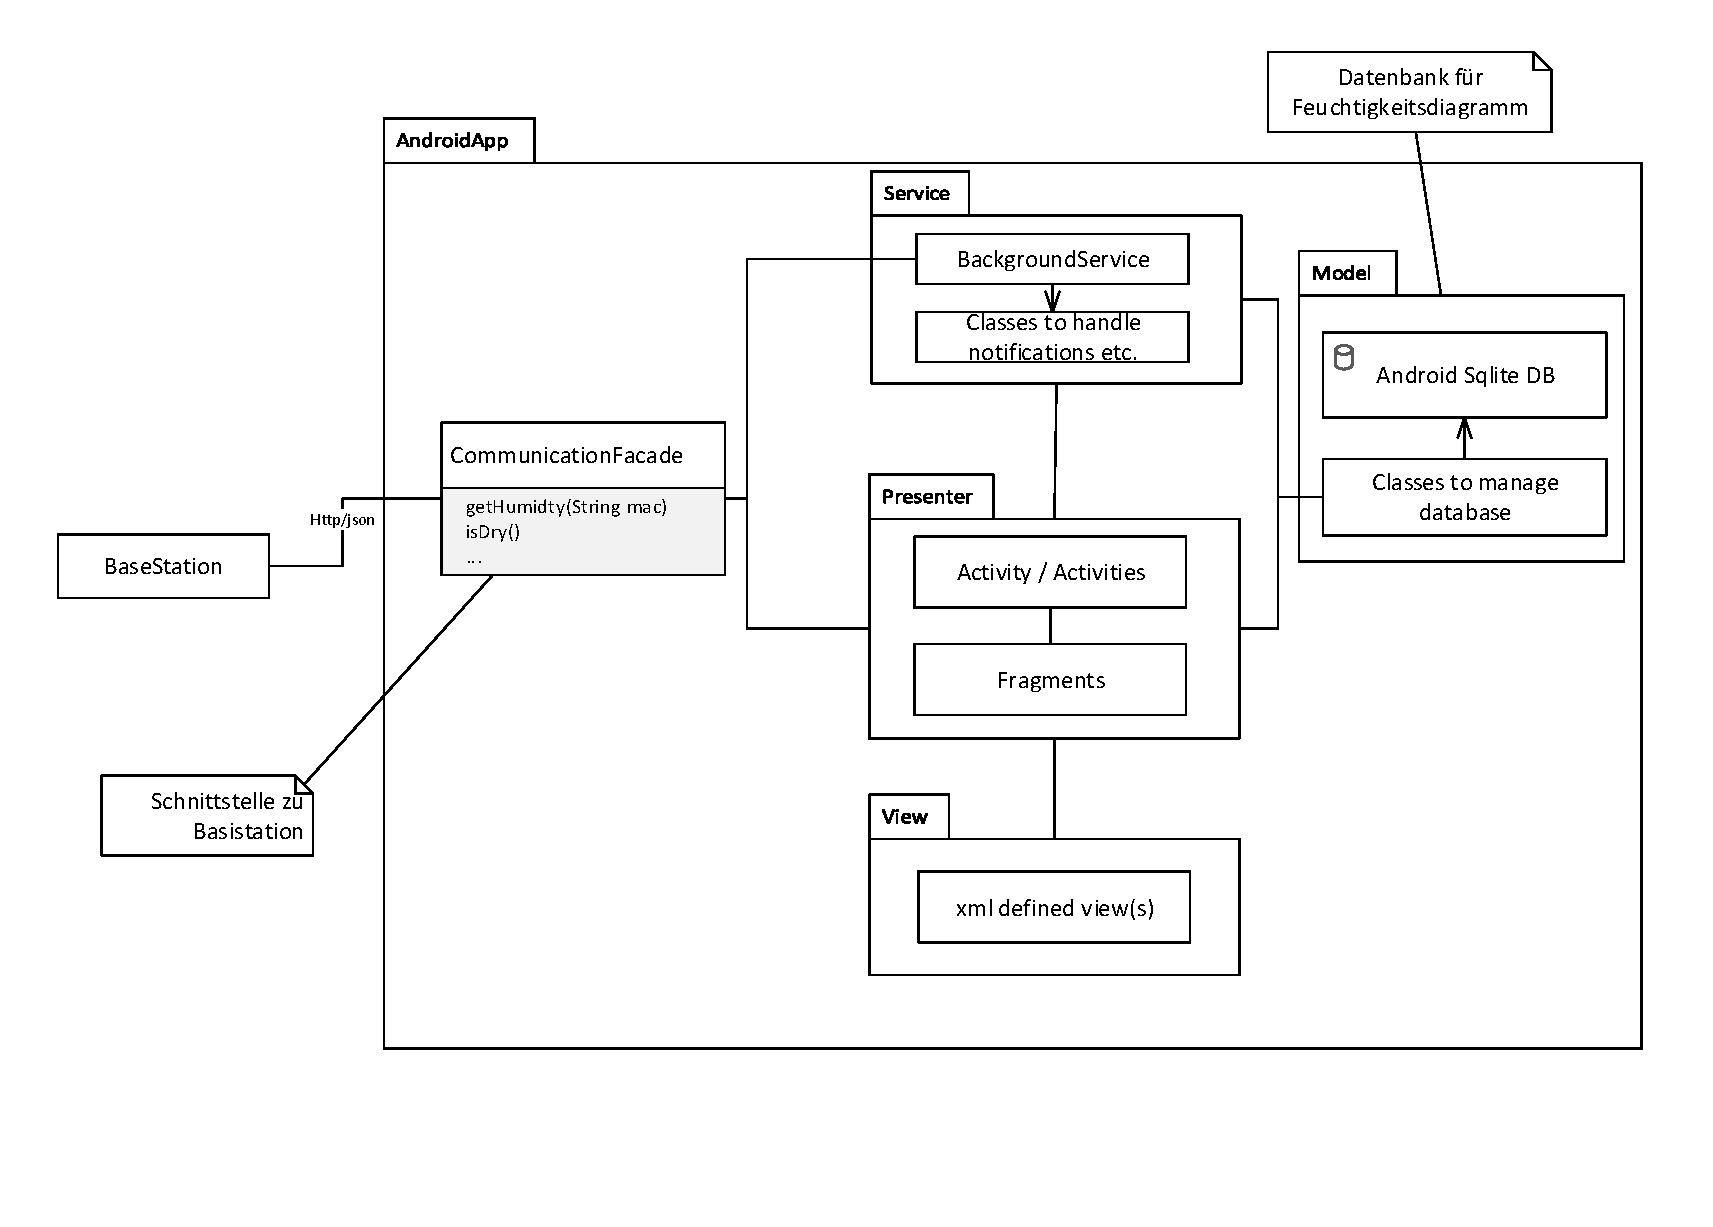
\includegraphics[scale=.6]{Architektur/App_v2.pdf} }
	\caption{Der Aufbau der Android-Applikation.}
\end{figure}
Die Android-Applikation bereitet die aus dem Sensor gewonnen Daten für den Benutzer grafisch auf und bietet darüber hinaus zusätzliche Funktionalitäten wie einen Alarm wenn die Wäsche den Status 'trocken' erreicht hat.\\
Sie kommuniziert über html/json mit der Basisstation, von welcher sie die Daten über Abfragen erhält. Unter den Aktivitäten ist neben dem aktuellen Status oder einem Interface zum Verbinden und Trennen von Sensoren auch ein Feuchtigkeitsdiagramm. Die Daten dafür werden in der internen SQLite-Datenbank gehalten. Zusätzlich registriert die App weitere Hintergrunddienste insbesondere für die Benachrichtigung wenn die Wäsche trocken ist.\\
Im folgenden sollen die Hauptbestandteile der App näher erläutert werden.

\begin{enumerate}
	\item[CommunicationFacade] CommunicationFacade ist eine Singleton Klasse welche als Kommunikationsschnittstelle für die komplette App dient. Sie enthält Methoden um Anfragen an die Basisstation zu stellen und Callback Interfaces um die Antworten entgegenzunehmen. Außerdem enthält sie eine Enumeration für Fehler die zurückgegeben werden können. Diese sind speziell für unsere Anwendung angepasst, so gibt es zum Beispiel einen Fehler für den Fall, dass kein Sensor mit der Basisstation verbunden ist.
	
	\item[DryRBackgroundService] Hierbei handelt es sich um ein Android Service eine Software Instanz die ohne eine App läuft. Dieser Service ist so konfiguriert, dass er sich beim Starten des Gerätes startet und wenn er beendet werden sollte sich automatisch neu startet. Der Service fragt regelmäßig die Feuchtigkeit und den Wäschestatus ab und speichert die Daten in einer Datenbank. Falls die Wäsche trocken ist wird dem Nutzer eine entsprechende Benachrichtigung angezeigt. Der Service kann von der App aus mit einem Singleton namens DryRBackgroundServiceProvider erreicht werden.
	
	\item[Presenter] In der Applikation gibt es diverse Klassen die als Presenter agieren. Sie haben Zugriff auf entsprechende nach Android Standard in XML definierte Views um Daten anzuzeigen und benutzen falls nötig die CommunicationFacade und die Datenbank um Daten abzufragen. Zum einen gibt es Activities und es gibt Fragmente, Activities stellen ein Fenster dar um etwas anzuzeigen und mit dem Nutzer zu interagieren. Fragmente sind ähnlich nur haben sie kein eigenes Fenster sondern müssen innerhalb einer Activity angezeigt werden. In unserer Anwendung haben wir eine MainActivity die verschiedene Fragmente anzeigt und zwischen diesen wechseln kann (Mittels Navigationsrichtlinien von Materialdesign umgesetzt). Außerdem gibt es eine DryRPreferenceActivity die die Einstellungen handhabt und bei Bedarf durch die MainActivity gestartet wird. Die Fragmente stellen die Hauptansichten der App dar so gibt es Fragmente um den Sensorstatus und den Wäschestatus anzuzeigen.
	
	\item[Datenbank] Für die Datenbank wurde Android SQLite eingesetzt. Es werden abgefragte Feuchtigkeits- und andere Wäschestatusinformationen abgespeichert und bei Bedarf auch wieder gelöscht. Der Zugriff auf die Daten läuft über die entsprechenden *Table Klassen. Ein Observer Pattern wurde eingesetzt um das Feuchtigkeitsdiagramm über neue Daten in der Datenbank zu benachrichtigen.
	
	\item[configuration.xml] In res/values/configuration.xml findet sich eine XML Datei die die Konfiguration der App leichter machen soll. So können hier verschiedene Zeiten für die Aktualisierung diverser Daten eingestellt werden. Vor allem können hier aber Verbindungsinformation für die Basisstation konfiguriert werden, so zum Beispiel Hostname der Station, Protokoll, Servlet URLs und timeouts.
\end{enumerate}
Da Android diverse Eigenheiten hat wie zum Beispiel Lebenszeit und Kontrollflusssübergabe bei Activities und Fragmenten empfehlen wir, falls noch kein Vorwissen besteht, die Grundlagen auf \url{http://developer.android.com} nachzulesen.
